\section{Localization}

\begin{frame}{afstande mellem farver}

\centering
\tdplotsetmaincoords{60}{110}
\begin{tikzpicture}[scale=4,tdplot_main_coords]

%set up some coordinates 
%-----------------------
\coordinate (O) at (0,0,0);
\tdplotsetcoord{P1}{1.1}{60}{30}
\tdplotsetcoord{P2}{1.5}{40}{60}

%draw figure contents
%--------------------

%draw the main coordinate system axes
\draw[ultra thick,red,->] (0,0,0) -- (1,0,0) node[anchor=north east]{$r$};
\draw[ultra thick,green,->] (0,0,0) -- (0,1,0) node[anchor=north west]{$g$};
\draw[ultra thick,blue,->] (0,0,0) -- (0,0,1) node[anchor=south]{$b$};

\draw[-stealth,color=gray] (O) -- (P1);
\draw[-stealth,color=gray] (O) -- (P2);
\draw[-stealth,thick] (P1) -- (P2);

\draw (P1) node[anchor=west]{$C_1$};
\draw (P2) node[anchor=west]{$C_2$};

%draw projection on xy plane, and a connecting line
\draw[dashed, color=gray] (O) -- (P1xy);
\draw[dashed, color=gray] (P1) -- (P1xy);

\draw[dashed, color=gray] (O) -- (P2xy);
\draw[dashed, color=gray] (P2) -- (P2xy);

%\draw[dashed] (P1xy) -- (P2xy);
%\draw[dashed] (P2) -- (P2xy);


\end{tikzpicture}

\end{frame}

\begin{frame}{maksimal afstand}

$$dist_{C_aC_b} = \vert C_a - C_b \vert$$

$$w_{C_aC_b} = \begin{cases}
	0 &\text{hvis } dist_{C_aC_b} > \rho \\
	1 - \frac{dist_{C_aC_b}}{\rho} &\text{hvis } dist_{C_aC_b} \leq \rho
\end{cases}$$

\end{frame}

\begin{frame}

\begin{figure}
\centering
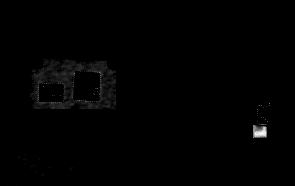
\includegraphics[scale=.7]{tracking/emptyGrid_TRACK2}


\includegraphics[scale=.7]{tracking/emptyGrid_TRACK}

\end{figure}
\end{frame}

\begin{frame}{Problemer med metoden}
\begin{itemize}
\item Støj
\item Farveændring (lys/skygge)
\item Opdateringshastighed
\end{itemize}

\end{frame}



\begin{frame}{Filtrering af støj}
3x3 Median filter \\


$$w'_{x,y} = \begin{cases}
	0 &\text{hvis } \vert V_{x,y} \vert < \rho \\
	w_{x,y} &\text{hvis } \vert V_{x,y} \vert \geq \rho
\end{cases}$$ \\
hvor $$V_{x,y} = \{w \in N_{x,y} \vert w > 0 \}$$
\end{frame}

\begin{frame}{Farveændring (lys/skygge)}
Løbende opdatering af sporingsfarve.
\begin{figure}
\centering

\includegraphics[scale=.7]{tracking/emptyGrid_FILTER}
\end{figure}

\end{frame}

\begin{frame}{Opdateringshastighed}
\begin{itemize}
\item reducere problemets størrelse.
\item robotten bevæger sig kun korte afstande mellem opdateringer.
\end{itemize}
\end{frame}

\begin{frame}
\begin{figure}
\centering

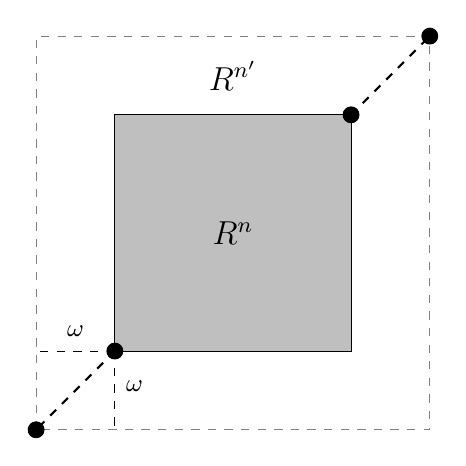
\begin{tikzpicture}[scale=.5]

%set up some coordinates 
%-----------------------
\coordinate (C1) at (0,0); % Outer top left
\coordinate (C2) at (10,10); % Outer bottom right
\coordinate (C3) at (2,2); % Inner top left
\coordinate (C4) at (8,8); % Inner bottom right

%draw figure contents
%--------------------

\draw [fill=lightgray] (C3) rectangle (C4); % Inner rectangle
\draw[dashed, color=gray] (C1) rectangle (C2); % Outer rectangle

\draw [fill] (C1) circle [radius=0.2]; % Outer top right
\draw [fill] (C2) circle [radius=0.2]; % Outer bottom left
\draw [fill] (C3) circle [radius=0.2]; % Inner top right
\draw [fill] (C4) circle [radius=0.2]; % Inner bottom left

\draw[thick,dashed] (C3) -- (C1); % Inner top right to outer top right
\draw[thick,dashed] (C4) -- (C2); % Inner bottom left to outer bottom left

\draw[dashed] (C3) -- (0,2);
\draw[dashed] (C3) -- (2,0);

\draw (5,5) node {\large $R^n$};
\draw (5,9) node {\large $R^{n'}$};

\draw (1,2.5) node {\small $\omega$}; % x1-w
\draw (2.5,1.1) node {\small $\omega$}; % y1-w

\end{tikzpicture}
\end{figure}

\end{frame}

\begin{frame}{Omregning fra punkt i billede til reelt punkt}

Insæt billede der viser ensvinklede trekanter.


\end{frame}








